%\renewcommand{\IMAGES}{\stpref/JET2PHI/IMAGES} %ye renuda
\renewcommand{\IMAGES}{./IMAGES} %ye renuda

\chapter{Particle-laden Wall Jet (JET\_P\_2PHI)}

\sousti{C. Caruyer - modified by Y. Eude (Renuda) le 18/06/2020}{18/06/2020}
\keywords{Particle-tracking, Lagrangian Simulation, Turbulent Flow, Two-way Coupling}

\section{Description}

The flow is a turbulent air jet along a vertical plane wall, laden with spherical glass particles. This configuration is one of the reference test-cases of the Workshop on two-phase flow predictions organised in Merseburg, Germany in 1996. It was also described in an article \cite{Sato1996}, and has been of previous numerical studies with former versions of \CS and with the in-house ESTET code \cite{validestetlag, Our_95}.

For the 1996-Merseburg workshop, three classes of particles were considered (140 $\mu$m glass particles, 50.3 $\mu$m nickel particles, and 49.3 $\mu$m glass particles) with different mass loads. The present numerical study focuses on the run involving 49.3 $\mu$m glass particles, and uses the particle-tracking (Lagrangian) module of \CS \cite{RefB-4}.


\subsection{Geometry and Inlet Conditions}

Tab.~\ref{inletcond} summarises the inlet conditions and the geometry of the domain; the geometry is represented in Fig.~\ref{geodom}.

\begin{table}[H]
\begin{center}
\begin{tabular}{|l|c|} \hline
Section width                             &   $150~mm$  \\ \hline
Section height                            &   $350~mm$  \\ \hline
Jet width $b$                             &   $5~mm$    \\ \hline
Maximum inlet velocity of the jet         &   $10~m.s^{-1}$  \\ \hline
Velocity of the co-current (unladen) flow &   $2~m.s^{-1}$   \\ \hline
Reynolds number for the jet               &   $3300$    \\ \hline
\end{tabular}
\end{center}
\caption{Inlet conditions}
\label{inletcond}
\end{table}

\newpage
\begin{figure}[H]
\centerline{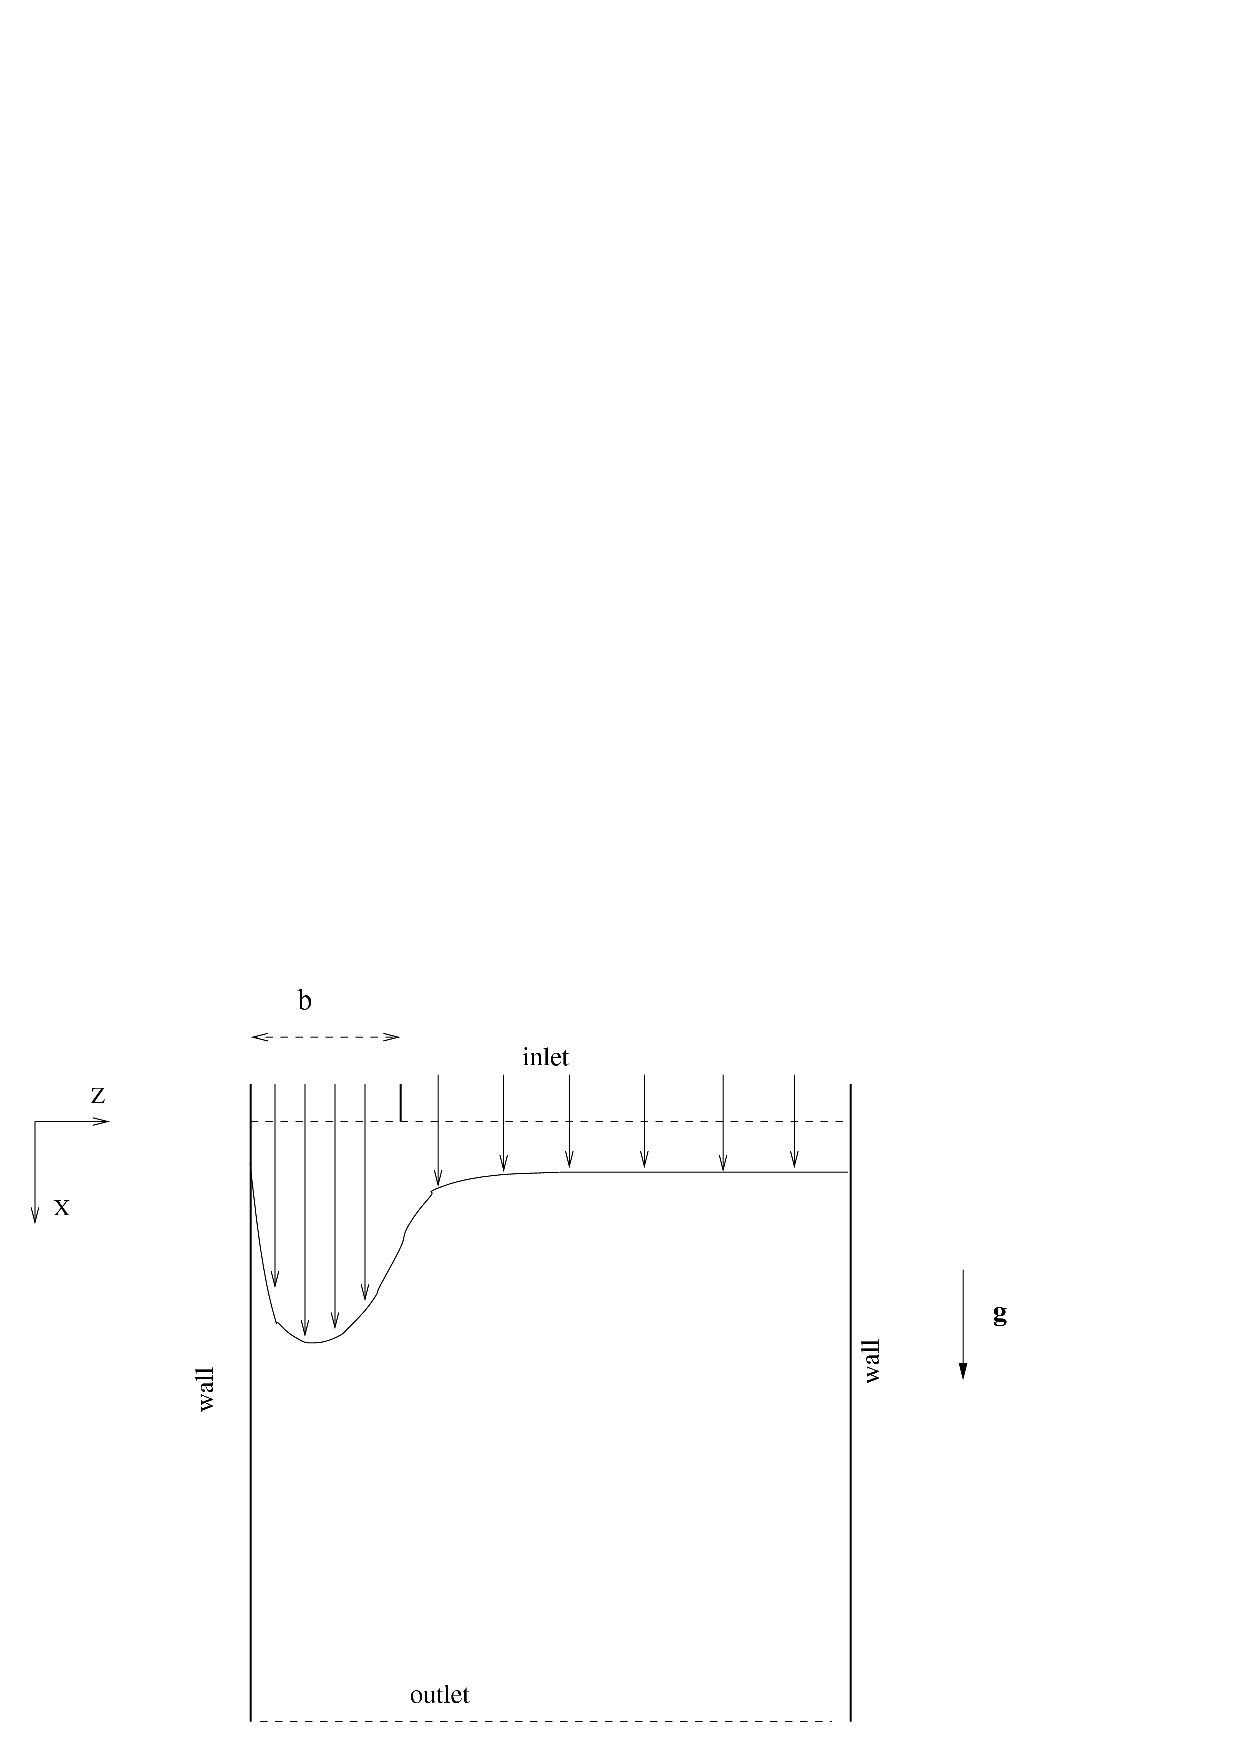
\includegraphics[width=8cm]{\IMAGES/geometry.png}}
\caption{{View of the geometry of the domain.}}
\label{geodom}
\end{figure}

\subsection{Physical Properties of the Fluid}

The fluid is air at room temperature.

% \begin{itemize}
% \item Dynamic viscosity: $\mu=1.6 \times 10^{-5}~kg.m^{-1}.s^{-1}$
% \item Density: $\rho=1.18~kg.m^{-3}$
% \end{itemize}

\subsection{Physical Properties of the Particles }

The particles injected are glass particles; the properties of the particle field are summarised in Tab.~\ref{tabpart}.

\begin{table}[H]
\begin{center}
\begin{tabular}{|l|c|} \hline
Mean diameter $d_{p}$                   &  \  $49.3~\mu m$         \\ \hline
Standard deviation of the diameter $\sigma_{p}$    &    $4.85~\mu m$          \\ \hline
Particles density $\rho_{p}$                 &    $2590~kg/m^{3}$       \\ \hline
Particle mass load $\phi$  \    &    $0.1$              \  \\ \hline
\end{tabular}
\end{center}
\caption{Particles properties}
\label{tabpart}
\end{table}


\subsection{Reference Publications}
\bibliographystyle{plain}
\bibliography{\stpref/STYLE/bibliography}

\section{Numerical Set-up}


\subsection{Mesh}


The mesh consists in one layer of 4646 hexaedra, and has been generated with the SIMAIL grid-generation software. It is represented in Fig.~\ref{mailla_jetpar} (global view and close-ups of the particle inlet zone). The normalised wall-normal distance of the boundary cell centers along the wall is approximately  ${y^+}~=~11$.

\begin{figure}[H]
\centerline{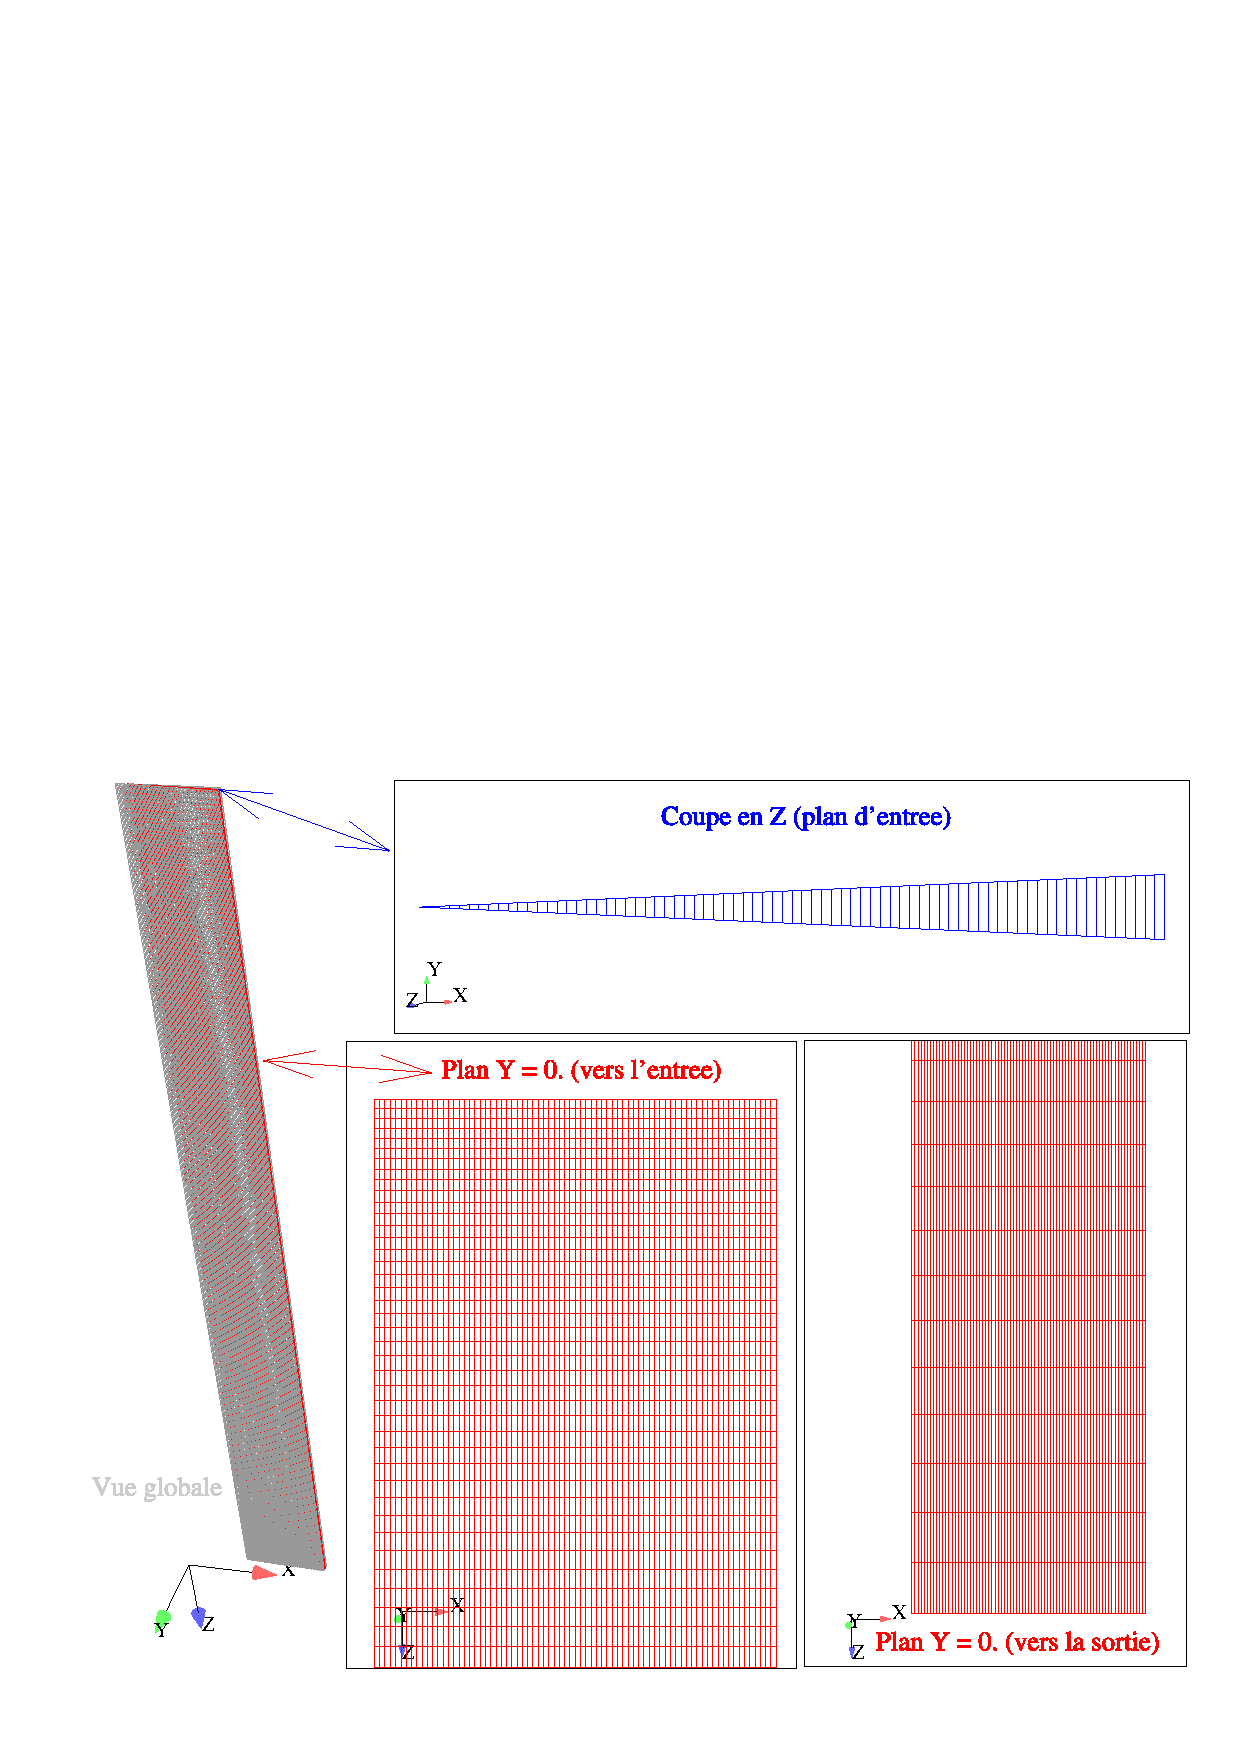
\includegraphics[width=10cm]{\IMAGES/maillage.png}}
\caption{\label{mailla_jetpar}{View of the mesh}}
\end{figure}

\newpage
\subsection{Boundary conditions}


% \subsubsection{Definition of the domain boundaries}

% Fig.~\ref{coul} represents the references given to each boundary face, and also provide the correspondence between the colors and the type of boundary conditions used for the air-flow.

% \begin{figure}[!ht]
% \centerline{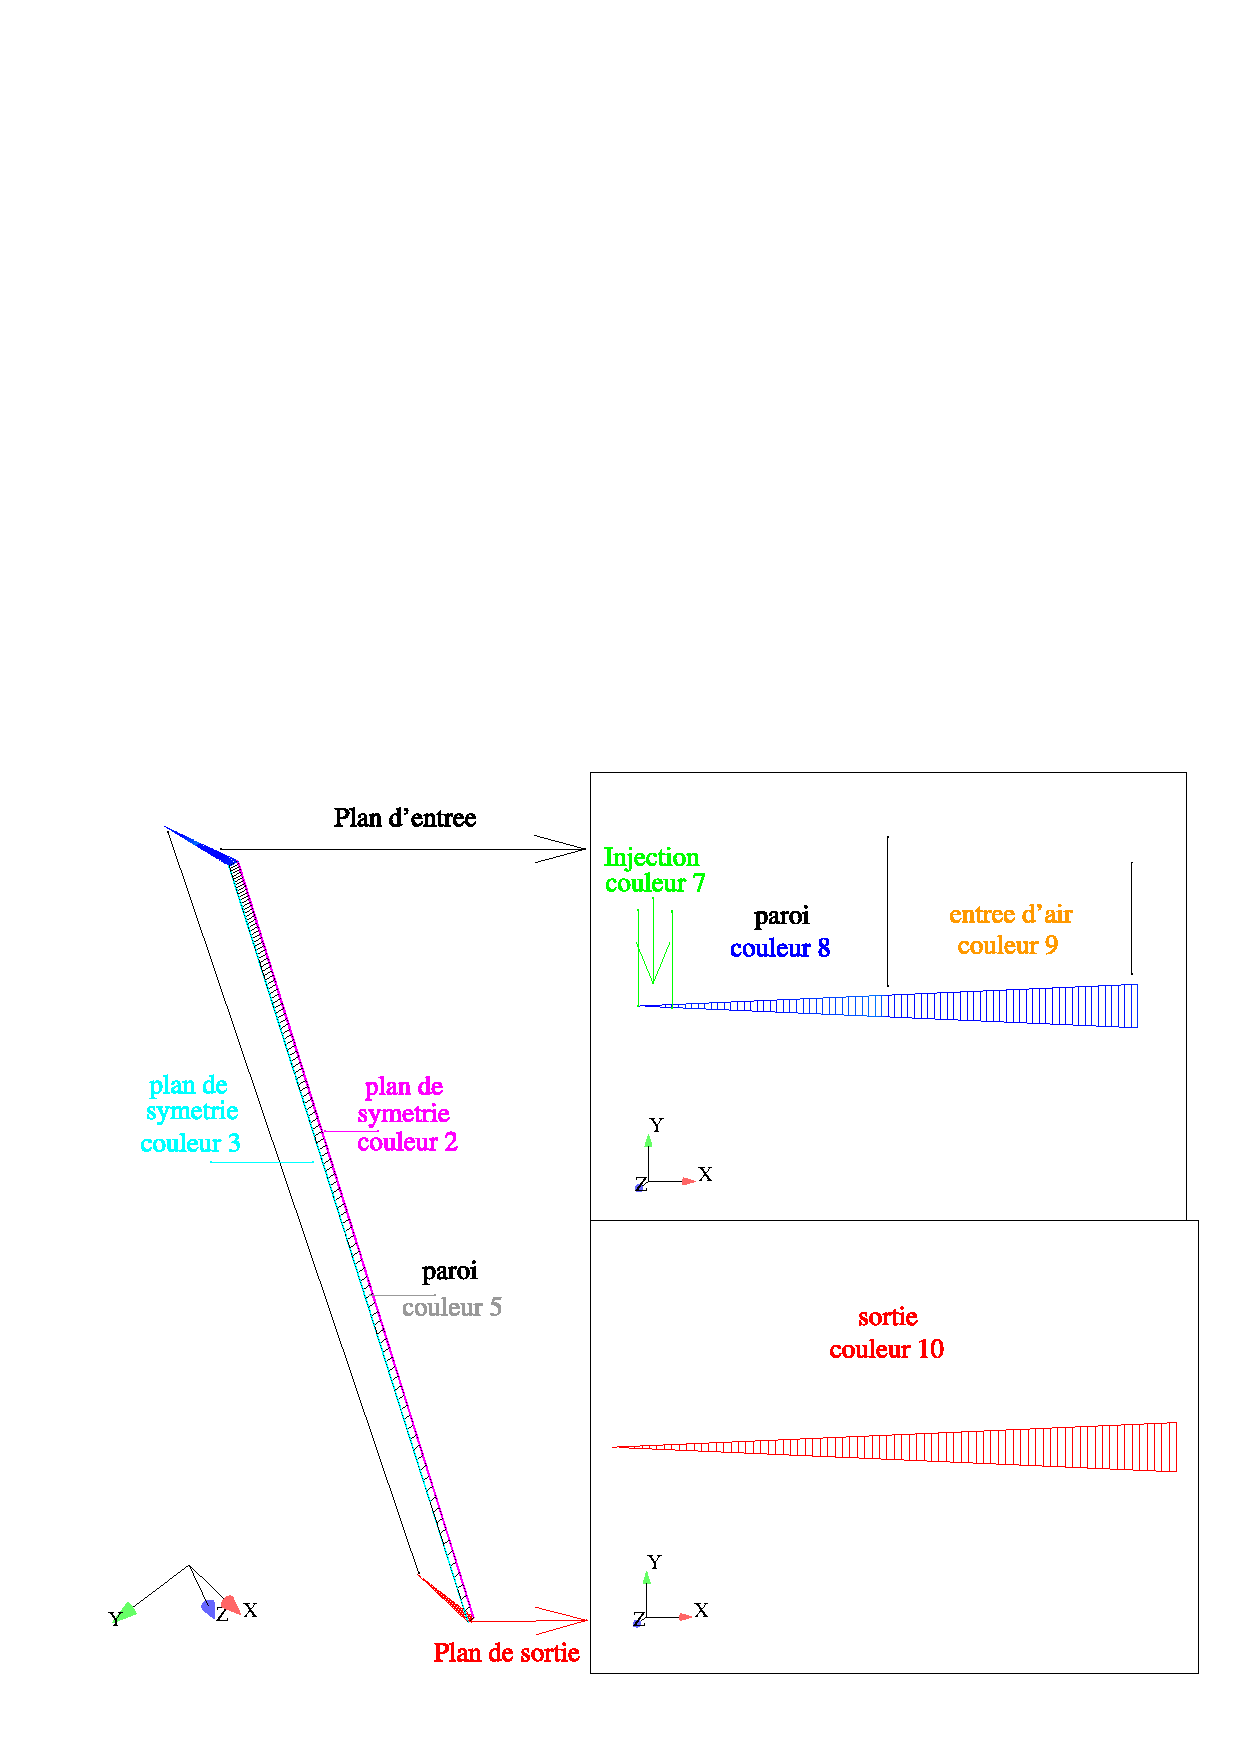
\includegraphics[width=6cm]{\IMAGES/couleur.png}}
% \caption{\label{coul}{References given to the boundary faces}}
% \end{figure}


\subsubsection{Boundary conditions for the air flow}

Tab.~\ref{CL_fluide} summarizes the characteristics of the air-flow injection given by the available experimental data, with respect to the transverse coordinate. In the numerical simulations, the last column (shear-stress) is not used.

\begin{table}[H]
\begin{center}
\begin{tabular}{|c|c|c|c|c|c|} \hline
 Coordinate & Mean  & Mean  &  Velocity & Velocity & shear-stress  \\
    $z$       & velocity & velocity   & fluctuation   &   &    \\
              & $<u>$   &  $<w>$    &  $u'$        &    $w'$    &  $<u'w'>$   \\
  \hline
      mm    &  $m.s^{-1}$   &   $m.s^{-1}$  & $m.s^{-1}$  &  $m.s^{-1}$ &$m^{2}.s^{-2}$\\ \hline
     0.8    & 8.568 &  0.290 & 0.733 & 0.168  &  0.0084 \\   \hline
     1      & 9.069 &  0.290 & 0.640 & 0.171  &  0.0048 \\   \hline
     1.2    & 9.521 &  0.324 & 0.455 & 0.139  & -0.0037 \\   \hline
     1.4    & 9.828 &  0.337 & 0.271 & 0.125  &  0.0017 \\   \hline
     1.6    & 9.850 &  0.345 & 0.211 & 0.122  &  0.0045 \\   \hline
     1.8    & 9.953 &  0.353 & 0.179 & 0.121  &  0.0043 \\   \hline
     2.0    & 9.944 &  0.361 & 0.170 & 0.119  &  0.0049 \\   \hline
     2.2    & 9.990 &  0.371 & 0.166 & 0.118  &  0.0043 \\   \hline
     2.4    & 9.958 &  0.365 & 0.189 & 0.120  &  0.0058 \\   \hline
     2.6    & 9.906 &  0.360 & 0.207 & 0.118  &  0.0077 \\   \hline
     2.8    & 9.798 &  0.355 & 0.254 & 0.121  &  0.0096 \\   \hline
     3.0    & 9.622 &  0.349 & 0.329 & 0.115  &  0.0131 \\   \hline
     3.2    & 9.494 &  0.349 & 0.402 & 0.136  &  0.0151 \\   \hline
     3.4    & 9.119 &  0.348 & 0.512 & 0.143  &  0.0199 \\   \hline
     3.6    & 8.578 &  0.328 & 0.531 & 0.143  &  0.0240 \\   \hline
     3.8    & 7.896 &  0.310 & 0.579 & 0.142  &  0.0244 \\   \hline
     4.0    & 7.081 &  0.278 & 0.592 & 0.156  &  0.0224 \\   \hline
     4.2    & 5.973 &  0.237 & 0.532 & 0.149  &  0.0307 \\   \hline
     4.4    & 4.821 &  0.179 & 0.513 & 0.159  &  0.0224 \\   \hline
     4.6    & 3.639 &  0.150 & 0.418 & 0.142  &  0.0167 \\   \hline
     4.8    & 2.001 &  0.069 & 0.296 & 0.174  &  0.0286 \\   \hline
     5.0    & 1.136 & -0.034 & 0.180 & 0.146  &  0.0191 \\   \hline
     5.2    & 0.821 & -0.024 & 0.140 & 0.116  &  0.0098 \\   \hline
     5.4    & 0.723 & -0.053 & 0.169 & 0.149  &  0.0164 \\   \hline
     5.6    & 0.736 & -0.063 & 0.162 & 0.136  &  0.0127 \\   \hline
     5.8    & 0.860 & -0.077 & 0.189 & 0.143  &  0.0144 \\   \hline
     6.0    & 1.037 & -0.086 & 0.184 & 0.142  &  0.0160 \\   \hline
     6.2    & 1.113 & -0.095 & 0.179 & 0.132  &  0.0139 \\   \hline
     6.5    & 1.309 & -0.060 & 0.183 & 0.117  &  0.0103 \\   \hline
     7.0    & 1.572 & -0.052 & 0.184 & 0.114  &  0.0079 \\   \hline
     7.5    & 1.711 & -0.054 & 0.169 & 0.107  &  0.0078 \\   \hline
     8.0    & 1.799 & -0.066 & 0.162 & 0.114  &  0.0103 \\   \hline
     8.5    & 1.882 & -0.045 & 0.137 & 0.097  &  0.0074 \\   \hline
     9.0    & 1.920 & -0.048 & 0.145 & 0.112  &  0.0110 \\   \hline
     9.5    & 1.948 & -0.054 & 0.131 & 0.111  &  0.0103 \\   \hline
    10.0    & 1.954 & -0.056 & 0.142 & 0.130  &  0.0139 \\   \hline
    11.0    & 1.995 & -0.046 & 0.136 & 0.124  &  0.0126 \\   \hline
    16.5    & 2.020 & -0.037 & 0.147 & 0.140  &  0.0170 \\   \hline
    21.0    & 2.011 & -0.041 & 0.141 & 0.140  &  0.0163 \\   \hline
    31.0    & 1.995 & -0.031 & 0.151 & 0.155  &  0.0203 \\   \hline
\end{tabular}
\end{center}
\caption{Inlet conditions of the air flow}
\label{CL_fluide}
\end{table}

\newpage
\subsubsection{Boundary conditions for the particle field}

Tab.\ref{CL_part} summarizes the characteristics of the particles injection given by the available experimental data. In the numerical simulations, the last column (shear-stress) is not used.


\begin{table}[H]
\begin{center}
\begin{tabular}{|c|c|c|c|c|c|c|} \hline
Coordinate  & Volume    & Velocity  & Velocity  & Velocity   & Velocity & shear-stress \\
   $z$      & Fraction  &  $u_p$   &   $w_p$  &  fluctuation  & fluctuation  &   \\
            &          &          &          &   ${u_p}'$  &  ${w_p}'$   & $<{u_p}'{w_p}'>$ \\
\hline
        mm  &           &  $m.s^{-1}$ &  $m.s^{-1}$  & $m.s^{-1}$  &  $m.s^{-1}$   & $m^{2}.s^{2}$\\   \hline
     $0   $ & $0.377 \times 10^{-4}$ & $5.544$ & {\em 0  }   & $0.352$ & $0.058 $ & $ 0.0017$\\   \hline
     $1   $ & $2.236 \times 10^{-4}$ & $8.827$ & {\em 0.179} & $0.352$ & $0.058 $ & $ 0.0017$\\   \hline
     $1.5 $ & $3.014 \times 10^{-4}$ & $9.068$ & {\em 0.206} & $0.275$ & $0.056 $ & $ 0.0016$\\   \hline
     $2.0 $ & $4.306 \times 10^{-4}$ & $9.169$ &{\em 0.221} & $0.252$ & $0.056 $ & $ 0.0027$\\   \hline
     $2.5 $ & $5.689 \times 10^{-4}$ & $8.923$ &{\em 0.220} & $0.367$ & $0.060 $ & $ 0.0077$\\   \hline
     $3.0 $ & $8.567 \times 10^{-4}$ & $8.295$ &{\em 0.223} & $0.516$ & $0.063 $ & $ 0.0146$\\   \hline
     $3.5 $ & $7.099 \times 10^{-4}$ & $7.151$ &{\em 0.206} & $0.657$ & $0.058 $ & $ 0.0206$\\   \hline
     $4.0 $ & $4.520 \times 10^{-4}$ & $6.048$ &{\em 0.190} & $0.872$ & $0.072 $ & $ 0.0447$\\   \hline
     $4.5 $ & $2.184 \times 10^{-4}$ & $4.785$ & {\em 0.195} & $1.080$ & $0.091 $ & $ 0.0752$\\   \hline
     $5.0 $ & $0.377 \times 10^{-4}$ & $5.544$ & {\em 0.504} & $0.792$ & $0.232 $ & $ 0.1145$\\   \hline
\end{tabular}
\end{center}
\caption{Particle inlet boundary conditions. The values of the particle inlet mean transverse velocity (emphasised values) are set to zero in our simulations.}
\label{CL_part}
\end{table}

{\bf Nota Bene} Like the former numerical studies with \CS and with the ESTET code, considering the uncertainties on the values of the particle mean transverse velocity $w_p$, it is chosen in the current study to set this inlet variable to zero.

\subsection{Physical modeling and numerical options}

A ``two-way'' coupling simulation is performed (with particle influence on the flow momentum and turbulent mean variables). The turbulent variables of the flow are resolved with the $k - \varepsilon$ ``linear production'' turbulence model. The inlet profiles are implemented through interpolations of experimental inlet variables in user-defined functions.

The parameters of the Lagrangian calculation are the following:
%
\begin{itemize}
\item[-] Complete model with turbulent dispersion and crossing trajectory effect (main direction of the flow: the x-axis) starting at the first Lagrangian iteration.
\item[-] Numerical scheme: first-order.
\item[-] Two-way coupling starting at the first Lagrangian iteration.
\end{itemize}

The time step is constant, uniform and set to $1 \times 10^{-4}$~s, sufficiently small to obtain a CFL number lower than 1 for the fluid, and so that the particles do not generally cross more than one cell during a time step. A single calculation is performed. The averaging of the relevant Lagrangian statistics begins from 2000 iterations (where the steady state is reached).


\section{Results obtained}


Fig.~\ref{volfrac} to Fig.~\ref{fluctrans} represent the numerical results obtained with \CS v6.0.2  compared the experimental data and to the results obtained with \CS v5.0.

\clearpage
\begin{figure}[H]
\centerline{\includegraphics[width=\textwidth]{\IMAGES/VNV/volume_fraction.pdf}}
\caption{{Transverse profile of the particle volume fraction at different elevations}}
\label{volfrac}
\end{figure}

\clearpage
\begin{figure}[H]
\centerline{\includegraphics[width=\textwidth]{\IMAGES/VNV/ver_velocity_average.pdf}}
\caption{{Transverse profile of the mean vertical particle velocity at different elevations}}
\label{meanver}
\end{figure}

\clearpage
\begin{figure}[H]
\centerline{\includegraphics[width=\textwidth]{\IMAGES/VNV/ver_velocity_fluc.pdf}}
\caption{{Transverse profile of the fluctuating vertical particle velocity at different elevations}}
\label{flucver}
\end{figure}

\clearpage
% \begin{figure}[p]
% \centerline{\includegraphics[width=\textwidth]{\IMAGES/trans_velocity_average.pdf}}
% \caption{{Mean transverse particle velocity}}
% \label{meantrans}
% \end{figure}

\clearpage
\begin{figure}[H]
\centerline{\includegraphics[width=\textwidth]{\IMAGES/VNV/trans_velocity_fluc.pdf}}
\caption{{Transverse profile of the fluctuating transverse particle velocity at different elevations}}
\label{fluctrans}
\end{figure}

